%
\section{The Fundamental Data Structures within StdRegions}
\label{sec:stdregions-datastructures}

In almost all object-oriented languages (which includes $C++$), there exists the concepts of {\em class attributes} and {\em object attributes}.  Class attributes are those attributes shared by all object instances (both immediate and derived objects) of a particular class definition, and object attributes (sometimes called data members) are those attributes whose values vary from object to object and hence help to characterize (or make unique) a particular object. In $C++$, object attributes are specified a header file containing class declarations; within a class declaration, attributes are grouped by their accessibility: {\em public} attributes, {\em protected} attributes and {\em private} attributes.  A detailed discussion of the nuances of these
categories are beyond the scope of this guide; we refer the interested reader to the following books for further details:  \cite{BStroustrup,SMeyers}.
For our purposes, the main thing to appreciate is that categories dictate access patters within the inheritance hierarchy and to the ``outside" world 
(i.e. access from outside the object).  We have summarized the relationships between the categories and their accessibility in Tables
\ref{table:publicinheritance}, \ref{table:protectedinheritance} and \ref{table:privateinheritance} \footnote{These tables are based upon information provided at http://www.programiz.com/cpp-programming/public-protected-private-inheritance, accessed 6 April 2018.}.


\begin{table}[ht]
\begin{center}
\caption{Accessibility in Public Inheritance}
\begin{tabular}{c c c c}
\hline\hline
Accessibility & private variables & protected variables & public variables \\
\hline
Accessibility from own class? & yes & yes & yes \\
Accessibility from derived class? & no & yes & yes\\
Accessibility from 2nd derived class? & no & yes & yes\\
\end{tabular}
\end{center}
\label{table:publicinheritance}
\end{table}

\begin{table}[ht]
\begin{center}
\caption{Accessibility in Protected Inheritance}
\begin{tabular}{c c c c}
\hline\hline
Accessibility & private variables & protected variables & public variables \\
\hline
Accessibility from own class? & yes & yes & yes \\
Accessibility from derived class? & no & yes & yes \\
&&&(inherited as \\
&&&protected variable)\\
Accessibility from 2nd derived class? & no & yes & yes\\
\end{tabular}
\end{center}
\label{table:protectedinheritance}
\end{table}

\begin{table}[ht]
\begin{center}
\caption{Accessibility in Private Inheritance}
\begin{tabular}{c c c c}
\hline\hline
Accessibility & private variables & protected variables & public variables \\
\hline
Accessibility from own class? & yes & yes & yes\\
Accessibility from derived class? & no & yes & yes \\
& & (inherited as & (inherited as \\
& & private variable) &  private variable) \\
Accessibility from 2nd derived class? & no & no & no \\
\end{tabular}
\end{center}
\label{table:privateinheritance}
\end{table}

Within the StdRegions directory of the library, there exists a class inheritance hierarchy designed to try to encourage re-use of core
algorithms (while simultaneously trying to minimize duplication of code).  We present this class hierarchy in Figure \ref{stdregions:stdexpansiontree}.

\begin{figure}[htb]
\centering
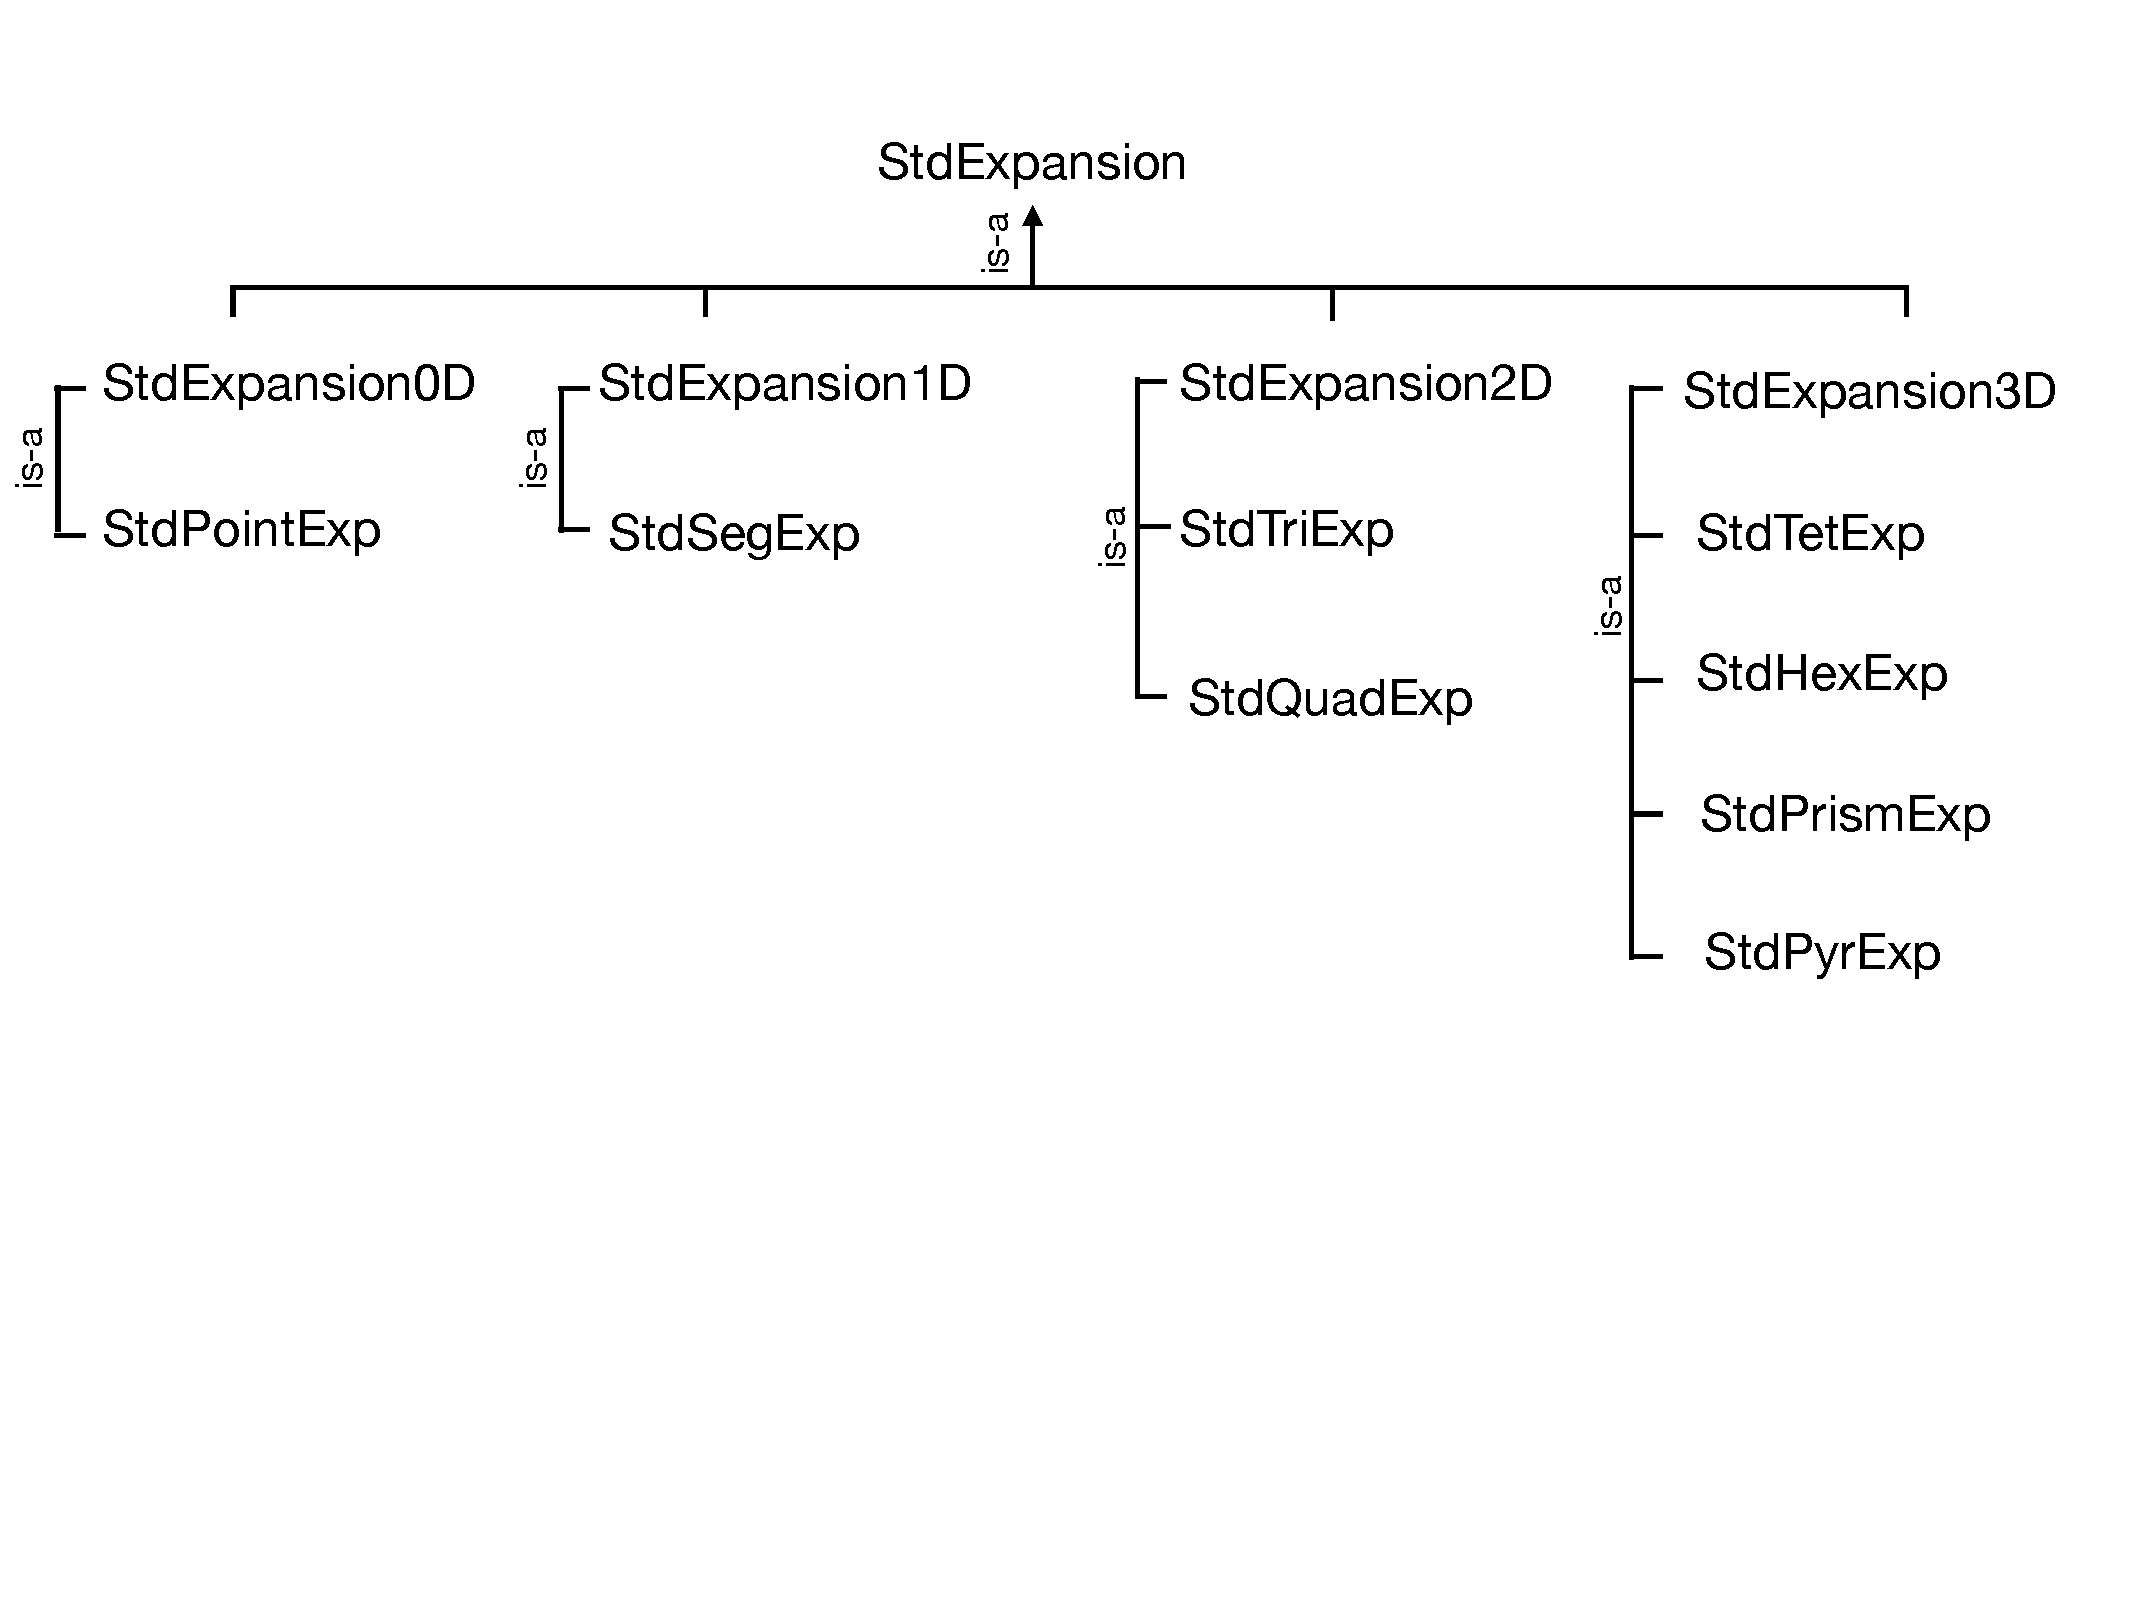
\includegraphics[width=6in]{img/stdexpansiontree.pdf}
\caption{Class hierarchy derived from StdExpansion, the base class of the StdRegions Directory.}
\label{stdregions:stdexpansiontree}
\end{figure}

As is seen in Figure \ref{stdregions:stdexpansiontree}, the StdRegions hierarchy consists of three levels:  the base level from which all
StdRegion objects are derived is StdExpansion.   This object is then specialized by dimension, yielding StdExpansion0D, 
StdExpansion1D, StdExpansion2D and StdExpansion3D.  The dimension-specific objects are then specialized based upon
shape.  

The object attributes (variables) at various levels of the hierarchy can be understood in light of Figure \ref{stdregions:stdexpansion}.
At its core, an expansion is a means of representing a function over a canonically-defined region of space evaluated at a collection of point positions.
The various data members hold information to allow all these basic building blocks to be specified.

\begin{figure}[htb]
\centering
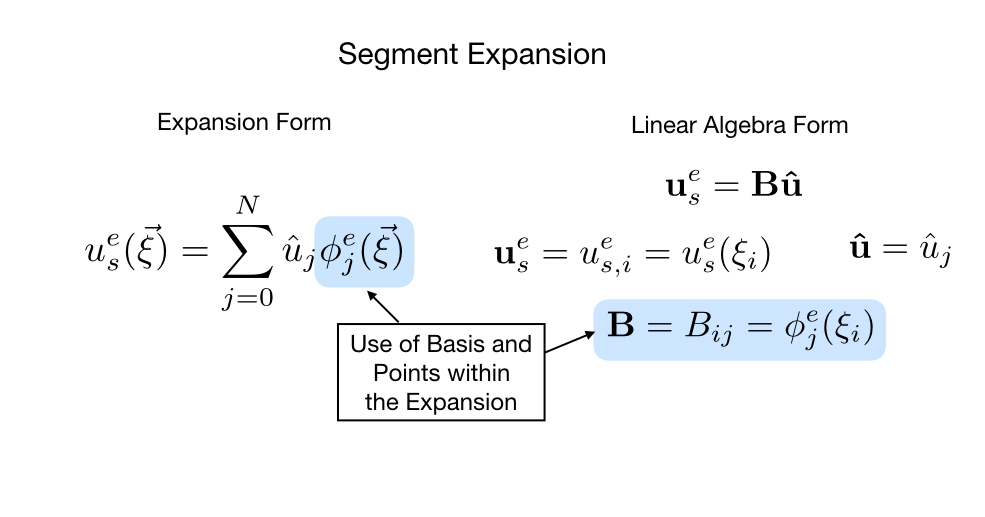
\includegraphics[width=6in]{img/StdExpansion.png}
\caption{Diagram to help understand the various data members (object attributes) contained within StdRegions and how they connect with the mathematical representation presented earlier.}
\label{stdregions:stdexpansion}
\end{figure}

The various private, protected and public data members contained within StdRegions are provided in the subsequent sections.

%%%%%%%%%%%%%%%%%%%%%%%%%%%%%%%%%%%%%%%%
\subsection{Variables at the Level of StdExpansion}

\paragraph{Private:}

There are private methods but no private data members within StdExpansion.

\paragraph{Protected:}

\begin{itemize}
\item  Array of Basis Shared Pointers:  \verb+m_base+
% 
\item  Integer element id: \verb+m_elmt_id+
%
\item Integer total number of coefficients in the expansion:  \verb+m_ncoeffs+
%
\item Matrix Manager: \verb+m_stdMatrixManager+
%
\item Matrix Manager: \verb+m_stdStaticCondMatrixManager+
%
\item IndexKeyMap Matrix Manager: \verb+m_IndexMapManager+
\end{itemize}


\paragraph{Public:}

There are public methods but no public data members within StdExpansion.



%%%%%%%%%%%%%%%%%%%%%%%%%%%%%%%%%%%%%%%%
\subsection{Variables at the Level of StdExpansion\$D for various Dimensions}

\paragraph{Private:}

There are private methods but no private data members within StdExpansion\$D.

\paragraph{Protected:}


\begin{itemize}
\item 0D and 1D: std::map<int, NormalVector> \verb+m_vertexNormals+
%
\item 2D: Currently does not have any data structure.  It should probably have \verb+m_edgeNormals+
%
\item 3D: std::map<int, NormalVector> \verb+m_faceNormals+
%
\item 3D: std::map<int, bool> \verb+m_negatedNormals+
\end{itemize}

\paragraph{Public:}

There are public methods but no public data members within StdExpansion\$D.

%%%%%%%%%%%%%%%%%%%%%%%%%%%%%%%%%%%%%%%%
\subsection{Variables at the Level of Shape-Specific StdExpansions}

\paragraph{Private:}

\paragraph{Protected:}

\paragraph{Public:}



